\section{Background}
\label{sec:cryptobinary-background}
%%%%%%%%%%%%%%%%%%%%

In this section, we provide background on and a classification of detection approaches that have been employed by existing tools to date.
%To our surprise, only a limited number of tools and approaches have been developed throughout the span of more than two decades.
\autoref{fig:cryptobinary-timeline} shows the evolution timeline of various techniques and approaches used in cryptographic function identification research whereas \autoref{fig:cryptobinary-tool_timeline} shows the development timeline of all studied tools.
We also provide an overview of some of the cryptographic features that existing tools focus on, to help better understand how they work and contextualize later discussion.

\begin{figure}[t]
  \centering
  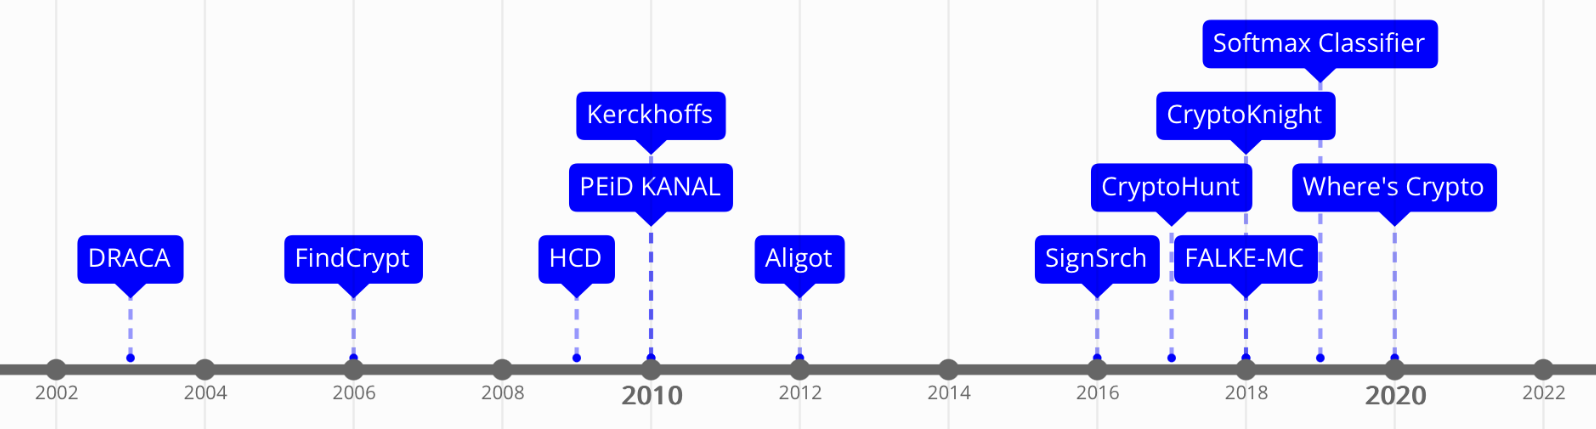
\includegraphics[width=0.95\textwidth,keepaspectratio]{ch-cryptobinary/figure/timeline.png}
  \caption{Timeline of the development of cryptographic algorithm detection tools}
  \label{fig:cryptobinary-tool_timeline}
\end{figure}

%%%%%%%%%%%%%%%%%%%%%%%%%%%%%%%%%%%%%%%%%%%%%%%%%%%%%%%%%%%%$$
\parhead{Cryptographic primitive vs. cryptographic function.} A brief note on notation used throughout this paper.  When we refer to a \textit{cryptographic function} or \textit{cryptographic algorithm}, we are generally referring to the entirety of a specific scheme or class of algorithms, such as RSA or hash functions.  When we say \textit{cryptographic primitive}, we generally mean a building block for a larger cryptographic scheme, such as a Feistel network.

%%%%%%%%%%%%%%%%%%%%%%%%%%%%%%%%%%%%%%%%%%%%%%%%%%%
\subsection{Categorization of Detection Approaches}
%%%%%%%%%%%%%%%%%%%%%%%%%%%%%%%%%%%%%%%%%%%%%%%%%%%
\label{sec:cryptobinary-detection}

Precision, scalability and performance of an identification approach all rely on the underlying techniques used.
Detection approaches can be divided into three categories:
i) Dynamic, ii) Static, and iii) Machine learning based approaches.

%%%%%%%%%%%%%%%%%%%%%%%%%%%%%%%%%

\parhead{Static Approaches.} Static approaches perform various forms of static analysis to detect
any static signatures, such as 'magic' constants, instruction sequences, and different code structures
such as S-boxes, as a means to identify cryptographic algorithms. This type of approach is based on the assumption that
cryptographic functions will perform a large number of arithmetic computations compared to non-cryptographic functions.
Harvey et al. \cite{harvey2001cipher} first proposed the idea of identifying cryptographic algorithms in binary files.
They focused on finding algorithms based on their constant
characteristics. By taking advantage of feature matching, subsequent
works \cite{lin2008automatic,caballero2007polyglot,wang2009reformat}
primarily focused on protocol reverse engineering. 
Chang et al. \cite{chang2014cryptographic} created a library of 3000 plus signature characteristics of cryptographic algorithms and also explored recognizing cryptographic algorithms based on Minimum Perfect Hash Function (MPHF).
Lestringant et al.~\cite{lestringant2015automated} used
data-flow isomorphism to find symmetric key algorithms.

Off-the-shelf tools such as Draft Crypto Analyzer
(DRACA)~\cite{draca}, Kanal~\cite{kanal}, Kerckhoffs~\cite{kerckhoffs},
Hash \& Crypto Detector (HCD)~\cite{hcd}, Signsrch~\cite{signsrch}, and Findcrypt~\cite{findcrypt2}, 
utilize static signature patterns of different cryptographic functions.
Static based approaches have low performance overhead. However, these
detection mechanisms can be easily bypassed using simple obfuscation techniques. For example,
the authors of Aligot~\cite{calvet2012aligot} showed that simple data obfuscation techniques
can bypass static analysis based detection mechanisms.

%%%%%%%%%%%%%%%%%%%%%%%%%%%%%%%%%%

\parhead{Dynamic Approaches.} Dynamic approaches~\cite{xu2017cryptographic,calvet2012aligot,li2012cipherxray}
primarily focus on identifying cryptographic primitives
from execution traces.
Lutz et al. \cite{lutz2008towards} first applied dynamic analysis to identify cryptographic algorithms based on three indicators:
i) presence of loops, ii) changes in entropy, and iii) high ratio of bitwise
arithmetic instructions.
Based on the data avalanche effect, CipherXRay~\cite{li2012cipherxray}
pinpoints the boundary of cryptographic operations and recovers transient
cryptographic secrets. However, this approach does not work in the case of stream
ciphers, for example, as they do not show any data avalanche effect.

Gr{\"o}bert et al.~\cite{grobert2011automated} proposed heuristic based 
approaches on both generic characteristics of cryptographic code and on
signatures for specific instances of cryptographic algorithms by mapping 
input-output (I/O) relations. Aligot~\cite{calvet2012aligot} further extends
this idea of I/O mapping. It retrieves
I/O parameters in an implementation-independent fashion, and compares
them with known cryptographic functions as well as performs
an interloop data flow analysis.
CryptoHunt~\cite{xu2017cryptographic} used bit-precise symbolic
loop mapping to identify cryptographic functions and applies guided fuzzing to
make the solution scalable. Park et al. \cite{park2020symmetric} proposed a hardware-assisted tracing technique to detect
symmetric-key cryptographic routines in anti-reverse engineered binaries via
recording the change of flow instructions from the CPU at run-time.
Dynamic approaches in general perform better than static based approaches in obfuscated
binaries, but suffer from much greater performance overhead.


%%%%%%%%%%%%%%%%%%%%%%%%%%%%%%%%%%%%%%%%%%%%%%%%% 

\parhead{Machine Learning Based Approaches.} With the growing popularity of machine learning, several recent works have explored utilizing such techniques.
Shin et al.~\cite{shin2015recognizing} discussed how recurrent neural networks can identify functions in binaries with greater accuracy and efficiency.
However, their approach was generalized for any function identification. 
For the purpose of cryptographic function identification,
Wright et al.~\cite{wright2009neural} proposed an artificial neural network model to classify
functional blocks as being either cryptographic or not by extracting the frequency of different logic instructions from a
disassembled program.
Benedetti et al. \cite{benedetti2017detection} used the `grap' tool to detect
cryptographic algorithms by creating patterns for AES and ChaCha20.
Falke~\cite{aigner2018falke} proposed a neural network based approach
by modeling classifiers for arbitrary cryptographic algorithms from
sample files and then automatically extracting features to train the neural
network. It offered a high detection rate in combination with
a low false positive rate.
Hill et al.~\cite{hill2018cryptoknight} proposed a Dynamic Convolutional Neural
Network based learning system (CryptoKnight) which learns from new cryptographic
execution patterns to classify unknown software.
Jia et al. \cite{jia2020neural} proposed an NLP-based approach which first extracts the
semantic information of assembly instructions and then transfers them into
100-dimensional vectors and later uses K-Max-CNN-Attention to classify
cryptographic functions.


%\parhead{Hybrid Solution.}
%\clg{This still needs to be filled out}


%\begin{figure}[h]
%	\includegraphics[width=\textwidth]{images/cryptoknight.pdf}
%	\caption{The CryptoKnight classification pipeline. 'Dynamic Binary Analysis' marked in red, is the point-of-failure.}
%\end{figure}


%The shared \texttt{CryptoTrace.so} object is built on the 32-bit \texttt{i386} architecture,
% and returns loading errors when run on \texttt{x86\_64} systems. 
 %On running the binary on an Ubuntu image running \texttt{i386}, d
 %ynamic instrumentation failed with segmentation faults, the stack trace displaying `\texttt{??? at CryptoTrace.so+0x7f550}' for every frame.


%\clg{This does not really seem relevant to the background section?  This seems like something that should maybe go in an appendix or something like that to explain why we couldn't test things?}

%\clg{I feel like background should maybe briefly introduce each tool, its techniques, and the algorithms it tries to target.  Or something like that.}
%\priyam{updated}


\subsection{Cryptographic Features}
\label{sec:cryptobinary-features}
%%%%%%%%%%%%%%%%%%%%%%%%%%%%%%%%
Cryptographic functions have their own (often quite distinct) set of characteristics, and work thus far has often leveraged these for identification, as they can lead to more tailored or performant techniques than general purpose binary analysis and code identification.
Many of these features only pertain to certain algorithms and cannot be used to identify others.
We now discuss some of the popular cryptographic features used for identification purposes.

%%%%%%%%%%%%%%%%%%%%%%%%%%%%
\parhead{Magic Constants.} In this approach, algorithm specific ``magic constants'' are searched for in the binary.  These are constant values that must occur in any implementation of a given algorithm.
%For example, the magic constants for the TEA algorithm usually are 2654435769 or
%0x9E3779B9. Existence of these constants in a binary can be used as a hint that it might contain TEA.
For instance, Signsrch~\cite{signsrch} relies on the magic number `0x9e3779b9' to detect the TEA algorithm; however, it fails to identify the algorithm when data obfuscation is applied~\cite{xu2017cryptographic}.

%%%%%%%%%%%%%%%%%%%%%%%%%%%%%%%%%
\parhead{Presence of Loops.} Most cryptographic functions use some form of loops for key generation, encryption, or other operations.
%For example, the factorization-based RSA algorithm has loops to perform modular exponentiation.
CryptoHunt~\cite{xu2017cryptographic} utilized loops as a means for detection. Given that loops may present in regular functions, further program analysis is necessary to ensure accurate detection.

%%%%%%%%%%%%%%%%%%%%%%%%%%%%%%%%%%
\parhead{Changes in Entropy.} The process of decryption usually decreases information entropy. Hence, entropy can be used as an indicator of  encrypted versus plaintext data. Several techniques~\cite{lutz2008towards, lee2022rcryptect} have used entropy to distinguish encrypted blocks from regular ones. 
However, relying on entropy can also lead to false positives in certain circumstances~\cite{grobert2011automated}.

%%%%%%%%%%%%%%%%%%%%%%%%%%%
\parhead{I/O Mapping.} Cryptographic functions sometimes have one-to-one mappings between their input to output, i.e., given a key and the plaintext, we might always get the same output, or given the input to a hash function, we should always get the same output. 
%These sort of unique one-to-one mappings can sometimes be used as indicators of the presence of cryptography (or even of specific deterministic algorithms like a hash function). 
However, these approaches rely on the accurate extraction of the key and input/output from the memory, as any wrong extraction can defeat the usefulness of unique mapping.
%data obfuscation
 
%%%%%%%%%%%%%%%%%%%%%%%%%%%%%%%%%%%%%
\parhead{Data-Flow Isomorphism.}
%A Data-Flow Graph (DFG) is a graph that represents data dependencies between a number of
%perations within a program~\cite{DFG}.
In this approach~\cite{lestringant2015automated}, a Data-Flow Graph (DFG)~\cite{DFG} is generated from the
corresponding assembly code, and subgraphs in the DFG are checked to see
whether they are isomorphic to the graph signature of a particular cryptographic
algorithm.
%This approach was first proposed by Lestringant
%et al~\cite{lestringant2015automated} and primarily used to identify symmetric
%key based algorithms. 
However, this approach is limited in the case of conditional
statements, which are more prominent in asymmetric algorithms. Additionally, DFG can
vary in effectiveness depending on data obfuscations techniques used in the implementation, such as data-splitting.

%%%%%%%%%%%%%%%%%%%%%
\parhead{S-Box.} Substitution boxes (S-Box)~\cite{sbox} are a fundamental component used in many symmetric key ciphers.
%An S-box is a table or function that swaps input bits with different bits, enhancing encryption security against attacks
%like differential and linear cryptanalysis, and often has a very distinct signature. 
For instance, the BLOWFISH algorithm
is a 64-bit block cipher that has an S-Box consisting of 1024 elements~\cite{jia2020neural} which are usually
sequentially stored in memory, allowing tools to detect BLOWFISH by locating this S-Box in memory. Similar techniques can be applied to Permutation Boxes (P-Box)~\cite{pbox}, which are methods of bit-shuffling to permute or transpose bits across S-box inputs.


%%%%%%%%%%%%%%%%%%%%%%%%%%%%%%%%%%%%
\parhead{Instruction Sequences.} An instruction sequence is a series of instructions or commands that a CPU executes in a specific order to perform tasks within a program. %These instructions can range from simple arithmetic calculations to more complex data manipulation and control flow operations. 
Many fundamental cryptographic operations will consist of fingerprintable instruction sequences and hence can be used for the purpose of identification. Nevertheless, this method may lose its effectiveness when dealing with control-flow obfuscations such as control-flow flattening~\cite{cfg_f}.




\subsection{Applications with Modern Cryptographic Algorithms}

Transport Layer Security (TLS) is a cryptographic protocol that is specifically crafted to facilitate secure communication over networks.

Starting from TLS 1.1, elliptic curve cryptography (ECC) has been incorporated into the TLS protocol. Furthermore, in TLS 1.3, ECC takes a central role in the base specification, featuring new signature algorithms, while RSA support has been discontinued. As of 2021, the deprecation of TLS 1.0 and 1.1 has taken place, resulting in ECC as the major choice for TLS ciphersuites.

There are numerous libraries that implement TLS, including OpenSSL, cryptlib, and Java Secure Socket Extension. Concurrently, beyond the TLS, a number of other applications leverage modern cryptographic algorithms. Notable examples include iMessage and Signal, both of which implement end-to-end encryption for enhanced security.

